\subsection{Camera-space burn progression}
The first shell event can involve very little of the material that a camera sees. To quantify this distinction, project all 34,687 foreground Gaussians into two calibrated cameras from the original woodpile capture and evaluate their depth-ordered opacity contributions at $470\times264$ pixels. For a fixed view, sum each site's front-to-back transmittance times its alpha over pixels. The denominator is the total weight of initially eligible shell sites; the numerator is the weight of those that have ignited by a particular frame. This is a reference-material matte. Gas emission, smoke, animated shading and scene elements outside the foreground are excluded. A fixed camera can reuse its weights. Constructing and checking one matte took 0.78--0.80 s in an offline implementation.

\begin{figure*}[t]
\centering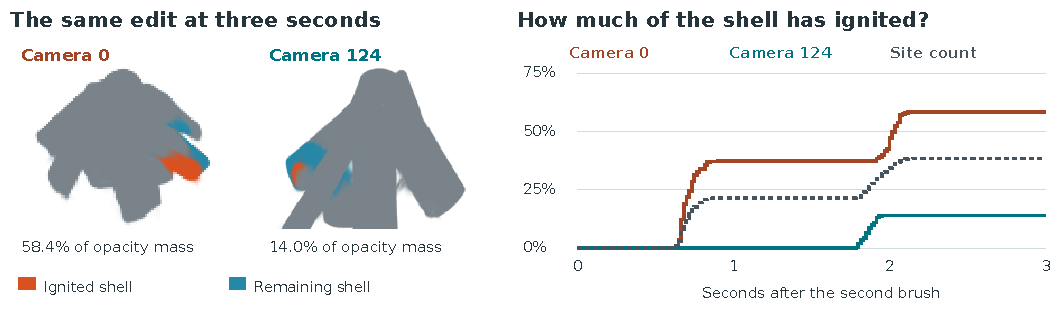
\includegraphics[width=.96\textwidth]{burn-progression.pdf}
\caption{Two calibrated views of the same A/B woodpile edit. The foregrounds are cropped and enlarged from their fixed reference cameras. Color distinguishes the initially eligible shell that has ignited by three seconds from its remaining material. The curves show cumulative fractions of initial shell mass or site count. One camera crosses one quarter at frame $+44$ and the other stays below one quarter through $+180$.}
\Description{Two gray woodpile silhouettes show burnt orange and remaining teal material. Opacity-weighted curves for the same edit finish at 58.4 and 14.0 percent, with the site-count curve between them.}
\label{fig:progress}
\end{figure*}

On A/B the first site ignited at $+36$. It contributed 0.009\% of eligible mass in camera 0. This view crossed one quarter at $+44$. Camera 124 reached only 13.96\% by $+180$ (Fig.~\ref{fig:progress}). Giving all sites equal weight would put the quarter crossing at $+111$ for both views. On B/A the first site crossed at $+50$, the site-count quarter at $+81$, and the opacity quarter at $+86$ and $+109$. Camera 124 saw only 4.16 pixel equivalents of eligible B/A material. These two retrospective trajectories distinguish the outputs; whether an artist requires the quarter-mass threshold remains open.
